\documentclass[aspectratio=169, 10pt]{beamer}
\usetheme{gotham}
\usetheme{pwr}

\gothamset{
    numbering=none,
    partframe default=off,  % Disable the display of the the part frame
    subsectionframe default=off,  % Disable the display of the subsection frame
    parttocframe default=off,  % Disable the display of the table of content frame after the part frame
    sectiontocframe default=off,  % Disable the display of the table of content frame after the section
    subsectiontocframe default=off,  % Disable the display of the table of content frame after the subsection
    progressbar style=fixed circle,
    % sectionframe template=gotham progressvert,
}


% -------------------- Language Customization --------------------
\figureName{MyFigure}  % Custom figure name
\tableName{MyTable}  % Custom table name


% -------------------- Title Slide Information --------------------
\title{Artifficial Intelligence in test smell detection}
\author{Jan Kowalski}
\institute{
    \vspace{2.5cm}
    Wrocław University of Science and Technology\\
    Advanced Topics in Artifficial Intelligence
}
\date{01.05.2025}


% -------------------- Footer Customization --------------------
\footerLeft{\insertauthor}  % Left part of the footer - can be blank
\footerMiddle{Advanced Topics in AI}  % Middle part of the footer - can be blank
\footerRight{\insertframenumber/\inserttotalframenumber}  % Right part of the footer - can be blank


% -------------------- Set logo / logos --------------------
\renewcommand{\gothamInstituteLogoSquare}[1][2ex]{
    
\includegraphics[height=0.7cm]{logos/pwr_logo.png}

    % Use the following command to include 2 logos, one next to each other
    % 
\includegraphics[height=0.7cm]{logos/pwr_logo.png} \hspace{0.35cm}
    % 
\includegraphics[height=0.7cm]{logos/wit_logo.png}
}


\begin{document}

% -------------------- Title Slide --------------------
\begin{frame}[nofootline]
    \maketitle  % Generates the title slide
\end{frame}


\begin{frame}[nofootline, standin]
    \vspace{0.5cm}
    \large \textbf{Table of contents}\\[2ex]
    \normalsize
    \tableofcontents  % Generates the table of contents
    \vspace{0.5cm}
\end{frame}


% -------------------- Rest of the presentation (content) --------------------
\section{Formatting and citations}
\begin{frame}{Slide with text formatting and citations}
    \lipsum[1][1-10]\cite{lipsum}\\[2.5ex]
    Another \textbf{text} \textit{with} \underline{citation} \cite{pontillo2024}.
\end{frame}


\section{Layout and code snippets}
\subsection{First example}
\begin{frame}[fragile]{Slide with 2 columns: text and small code snippets}
    \begin{columns}
    \centering
    \begin{column}{0.52\textwidth}
        \justifying
        \small
        \lipsum[1][4-6]\\[2.5ex]
        \lipsum[2][1-4]
    \end{column}
    \begin{column}{0.45\textwidth}
        \centering
        \scriptsize

        \begin{minted}{python}
my_list = [2, 5, 6]
my_list[len(my_list):] = [5]  # [2, 5, 6, 5]
        \end{minted}

        \vspace{2pt}
        \hrule
        \vspace{2pt}
        Appending to the list using slice assignment\\[5ex]

        \begin{minted}{python}
my_list = [2, 5, 6]
my_list.extend([-4])  # [2, 5, 6, -4]
        \end{minted}

        \vspace{2pt}
        \hrule
        \vspace{2pt}
        Appending to the list using \texttt{extend()}\\[5ex]


        \begin{minted}{python}
my_list = [2, 5, 6]
my_list.insert(len(my_list), 3)  # [2, 5, 6, 3]
        \end{minted}

        \vspace{2pt}
        \hrule
        \vspace{2pt}
        Appending to the list using \texttt{insert()}\\[5ex]

    \end{column}
\end{columns}
\end{frame}

\subsection{Second example}
\begin{frame}{Columnar layout with text only}
    \justifying
    \lipsum[1][1-5]\\[8ex]
  
    \begin{columns}
        \pause
        \centering
        \begin{column}{0.46\textwidth}
            \justifying
            Some key assumptions:
            \begin{itemize}
                \item \textit{\lipsum[1][6]}
                \item \textit{\lipsum[1][7]}
            \end{itemize}
            \vspace{0.2cm}
        \end{column}
        \pause
        \begin{column}{0.46\textwidth}
            \justifying
            \textbf{\lipsum[1][8-12]}
        \end{column}
    \end{columns}
\end{frame}


\subsection{Third example}
\begin{frame}[fragile]{Columnar layout with code snippets only}
    \begin{columns}
        \centering
        \begin{column}{0.46\textwidth}
            \scriptsize
            \begin{minted}[autogobble]{java}
                public class UserService {
                    public User createUser(User user) { ... }
                    public boolean validateEmail(String email) { ... }
                    public void sendWelcomeEmail(User user) { ... }
                    public void calculateUserStats() { ... }
                    public void generateReport() { ... }
                }
            \end{minted}
            \vspace{2.85cm}
        \end{column}

        \begin{column}{0.46\textwidth}
            \scriptsize
            \begin{minted}[autogobble]{java}
                public class UserService {
                    public User createUser(User user) { ... }
                    public User getUserById(String id) { ... }
                    public void updateUser(User user) { ... }
                    public void deleteUser(String id) { ... }
                }
                
                public class EmailService {
                    public void sendWelcomeEmail(User user) { ... }
                    public boolean validateEmail(String email) { ... }
                }
                
                public class ReportingService {
                    public void calculateUserStats() { ... }
                    public void generateReport() { ... }
                }
            \end{minted}
        \end{column}
    \end{columns}
\end{frame}


\section{Definitions}
\begin{frame}[fragile]{Slide with definitions}
    \begin{defbox}{Test smell \cite{pontillo2024}}
        Test smells are symptoms of sub-optimal design choices adopted when developing test cases.
    \end{defbox}
    \vspace{0.2cm}
    \begin{defbox}{Cumulative distribution function\cite{wiki:normal_dist}}
        The cumulative distribution function (CDF) of the standard normal distribution, usually denoted with the capital Greek letter $\Phi$, is the integral 
        \begin{equation}
            \Phi(x) = \frac{1}{\sqrt{2\pi}}\int_{-\infty}^{x}{e^{-t^2 / 2}dt}
        \end{equation}
    \end{defbox}
\end{frame}


\begin{frame}[fragile]{Slide with a pause}
    \lipsum[1][1-5]\\[2ex]
    \pause
    \justifying
    This text appears \textbf{after a pause}. \lipsum[1][6-15]
\end{frame}


\section{Images}
\subsection{One big image}
\begin{frame}[fragile]{Slide with 1 big image}
    \justifying
    \begin{figure}[!htbp]%
        \centering
        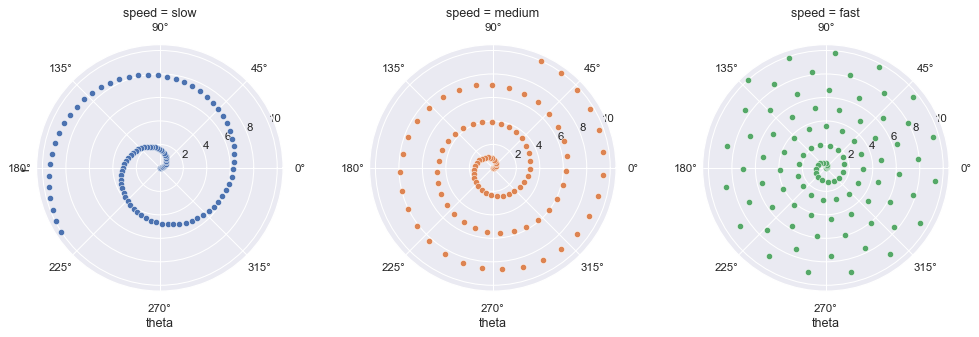
\includegraphics[width=0.9\textwidth]{images/radial_facets.png}
        \caption{FacetGrid with custom projection\\
        \tiny\url{https://seaborn.pydata.org/_images/radial_facets.png}}
    \end{figure}
\end{frame}


\subsection{Two smaller images}
\begin{frame}[fragile]{Slide with 2 smaller images}
    \begin{columns}
        \centering
        \begin{column}{0.44\textwidth}
            \vspace{0.3cm}
            \begin{figure}[!htbp]%
                \centering
                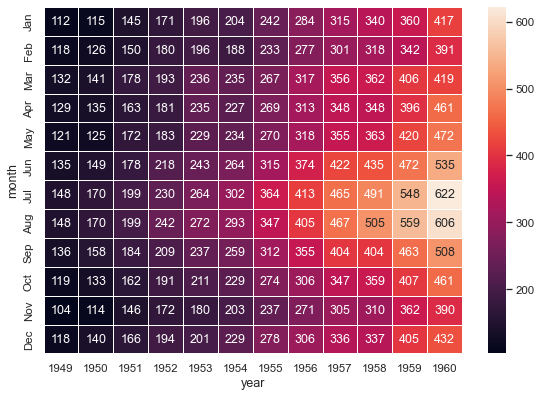
\includegraphics[width=0.9\textwidth]{images/spreadsheet_heatmap.png}
                \caption{Annotated heatmap\\
                \tiny\url{https://seaborn.pydata.org/_images/spreadsheet_heatmap.png}}
            \end{figure}
        \end{column}
        \begin{column}{0.44\textwidth}
            \begin{figure}[!htbp]%
                \centering
                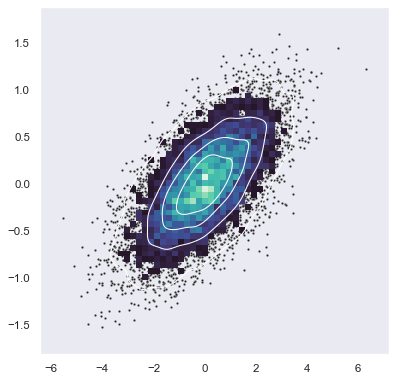
\includegraphics[width=0.75\textwidth]{images/layered_bivariate_plot.png}
                \caption{Bivariate plot with multiple elements\\
                \tiny\url{https://seaborn.pydata.org/_images/layered_bivariate_plot.png}}
            \end{figure}
        \end{column}
    \end{columns}
\end{frame}

{
    \AtBeginSection{}
    \section{Outro}
    \begin{frame}[nofootline, standout]
        \centering
        {\huge \textbf{Outro}}
        \vspace{15pt}
        \hrule
        \vspace{15pt}
        {\normalsize \textbf{If you have suggestions or improvements, please open an issue or pull request.}}
    \end{frame}
}
% \section{Q&A}
% \begin{frame}[nofootline, standout]
%     \centering
%     {\huge \textbf{Q&A}}
%     \vspace{15pt}
%     \hrule
%     \vspace{15pt}
%     \textbf{If you have suggestions or improvements, please open an issue or pull request.}
% \end{frame}


% -------------------- References (from the references.bib file) --------------------
\renewcommand{\bibsection}{}  % Removes a section creation on the references
\begin{frame}{References}
\bibliographystyle{plain}
\scriptsize
\bibliography{references}
\end{frame}

\end{document}


